\documentclass{report}[a4paper,12pt]
\usepackage[utf8]{inputenc}
\usepackage[frenchb]{babel}
\usepackage[T1]{fontenc}
\usepackage{graphicx}
\usepackage{array}
%\usepackage{fancyhdr}
\usepackage{listings}
%\pagestyle{fancy}
\usepackage{color}
%\definecolor{javared}{rgb}{0.6,0,0} % for strings
%\definecolor{javagreen}{rgb}{0.25,0.5,0.35} % comments
%\definecolor{javapurple}{rgb}{0.5,0,0.35} % keywords
%\definecolor{javadocblue}{rgb}{0.25,0.35,0.75} % javadoc
\definecolor{hellgelb}{rgb}{1,1,0.8}
\definecolor{colKeys}{rgb}{0,0,1}
\definecolor{colIdentifier}{rgb}{0,0,0}
\definecolor{colComments}{rgb}{1,0,0}
\definecolor{colString}{rgb}{0,0.5,0}
\lstset{%
language=ruby%
morekeywords={}%
float=hbp,%
basicstyle=\ttfamily\small, %
identifierstyle=\color{colIdentifier}, %
keywordstyle=\color{colKeys}, %
stringstyle=\color{colString}, %
commentstyle=\color{colComments}, %
columns=flexible, %
tabsize=2, %
frame=single, %
extendedchars=true, %
showspaces=false, %
showstringspaces=false, %
numbers=left, %
numberstyle=\tiny, %
breaklines=true, %
backgroundcolor=\color{hellgelb}, %
breakautoindent=true, %
captionpos=b%
}
\title{Projet Tuteurés -Outils de gestion centralisée de machines virtuelles\\\\Tuteur : Lucas Nussbaum}
\author{Sébastien Michaux - Augustin Bocca - Julien Tournois - Mathieu Lamouroux}
\date{\today}
\begin{document}
\maketitle
\begin{abstract}
%%%%%%%%%%%%%%%%%%%%%%
%% Résumé du projet %%
%%%%%%%%%%%%%%%%%%%%%%
\end{abstract}
\newline
\newline
\newline
\newline
\newline
\newline
\newline
\begin{center}
Remerciements
\\
Avant tout développement sur cette expérience, il apparait opportunt de commencer ce rapport par dess remerciements, à ceux qui nous on beaucoup appris au cours de cette période, et également à ceux qui ont eu la gentillesse de faire de ce projet un moment très profitable.\\
Aussi nous remercions Lucas Nussbaum, notre maître de stage qui nous a accompagné avec beaucoup de patience et de pédagogie. 
\end{center}

\newpage
\tableofcontents
\newpage
\chapter{Introduction}
\section{Présentation du projet}
%\paragraph{Objectif}
Mettre en place, évaluer et comparer différents outils permettant de gérer de manière
centralisée et automatisée une infrastructure basée sur des machines virtuelles: Ganeti,
OpenXenManager, virt-manager, Archipel...
\section{Introduction à la virtualisation}
\subsection{Machine virtuelle}


Une machine virtuelle est un conteneur isolé capable d'exécuter
ses propres système d'exploitation et applications.
Une machine virtuelle se comporte exactement comme un ordinateur physique
et contient ses propres processeurs, mémoire RAM, disque dur et carte
d'interface réseau virtuels.Une machine virtuelle
a pour but de générer sur une même machine un ou plusieurs environnements
d'exécution applicative. On en distingue deux types d'application
: d'une part la virtualisation par le biais d'un hyperviseur jouant
le rôle d'émulateur de système (PC ou serveur), d'autre part la virtualisation
applicative qui permet de faire tourner un application sur un poste
client quelque soit le système sous-jacent.

\subsection{Hyperviseur }


La machine virtuelle avec hyperviseur est utilisée pour générer au
dessus d'un système d'exploitation serveur, une couche logicielle sous
la forme d'un émulateur permettant de créer plusieurs environnements
d'exécution serveur. Cet émulateur se place comme un niveau supplémentaire qui se greffe sur le système d'origine.
\newpage
\subsection{Enjeux de la virtualisation}


Actuellement, les entreprises rencontrent des besoins qui ne sont
pas couverts.

Au niveau de la sécurité, les entreprises souhaiteraient isoler les
services sur des serveurs différents. Pour la maintenance, il serait
utile d'améliorer des services tels que la disponibilité, la migration,la redondance,la flexibilité ou le temps de réponse. Il serait également bienvenu de tester, déléguer l'administration d'un système ...


Une des solutions pour répondre à ces besoins serait d'acquérir davantage de plateformes de travail.


La multiplications des serveurs pose cependant un certain nombre
de problème, augmenter sans cesse son parc informatique est impossible
pour plusieurs raisons : 
\begin{itemize}
\item Tout d'abord au niveau écologique cela entrainerait un surplus de déchets électronique,une consommation d'energie directe et de l'énergie utilisée pour refroidir les salles serveur.
\item Au niveau de la surface utilisée, les salles machine seraient vite encombrées, puis apparaitra des problèmes tel que la nuisance sonore, le manque de puissance pour alimenter les salles serveur. 
\item Au niveau économique les couts d'achat, de recyclage, de fonctionnement, de maintenance seraient trop chère. La mise en place de serveur de virtualisation est une solution pour résoudre ces problèmes.
\end{itemize}

Le but de la virtualisation est de donner un environnement système
au programme pour qu'il croie être dans un environnement
matériel. Pour cela, une machine virtuelle est utilisée. Ainsi, plusieurs
environnements d'exécution sont créés sur une seule
machine, dont chacun émule la machine hôte. L'utilisateur
pense posséder un ordinateur complet pour chaque système d'exploitation
alors que toutes les machines virtuelles sont isolées entre elles.

\subsection{Histoire de la virtualisation}

La virtualisation est un concept qui a été mis au point pour la première
<<<<<<< HEAD
fois dans les années 1960 pour permettre la partition dune vaste gamme de matériel mainframe et optimiser l'utilisation du matériel. De nos jours, les ordinateurs basés sur l'architecture x86 sont confrontés aux mêmes problèmes de rigidité et de sous-utilisation que les mainframes dans les années 1960. VMware a inventé la virtualisation pour la plate-forme x86 dans les années 1990 afin de répondre notamment aux problèmes de sous-utilisation, et a surmonté les nombreux défis émergeant au cours de ce processus. Aujourd'hui, VMware est devenu le leader mondial de la virtualisation x86 avec plus de 190 000 clients, dont la totalité des membres du classement Fortune 100.

=======
fois dans les années 1960 pour permettre la partition d'une vaste gamme de matériel mainframe et optimiser l'utilisation du matériel. De nos jours, les ordinateurs basés sur l'architecture x86 sont confrontés aux mêmes problèmes de rigidité et de sous-utilisation que les mainframes dans les années 1960. VMware a inventé la virtualisation pour la plate-forme x86 dans les années 1990 afin de répondre notamment aux problèmes de sous-utilisation, et a surmonté les nombreux défis émergeant au cours de ce processus. Aujourd'hui, VMware est devenu le leader mondial de la virtualisation x86 avec plus de 190 000 clients, dont la totalité des membres du classement Fortune 100.
\newpage
>>>>>>> 890b8536ca977898c0a36d608fa5a6da1fadd342
\subsection{Au commencement, la virtualisation des mainframes}

La virtualisation a été mise en œuvre pour la première fois il y
a plus de 30 ans par IBM pour partitionner logiquement des mainframes
en machines virtuelles distinctes. Ces partitions permettaient un
<<<<<<< HEAD
traitement « multitâche », à savoir l exécution simultanée de plusieurs applications et processus. Étant donné que les mainframes consommaient beaucoup de ressources en même temps, le partitionnement
constituait un moyen naturel de tirer pleinement parti de l investissement matériel.
\newpage
=======
traitement « multitâche », à savoir l'exécution simultanée de plusieurs applications et processus. Étant donné que les mainframes consommaient beaucoup de ressources en même temps, le partitionnement
constituait un moyen naturel de tirer pleinement parti de l'investissement matériel.

>>>>>>> 890b8536ca977898c0a36d608fa5a6da1fadd342
\section{Présentation de Grid5000}
\begin{figure}
\begin{center}

\includegraphics{images/logo.png}
\caption{Logo de Grid5000}
\end{center}

\end{figure}
Aujourd’hui, grâce à Internet, il est possible
d’interconnecter des machines du monde entier pour
traiter et stocker des masses de données. Cette collection
hétérogène et distribuée de ressources de stockage et de
calcul a donné naissance à un nouveau concept : les
grilles informatiques.

L’idée de mutualiser les ressources
informatiques vient de plusieurs facteurs, évolution de la
recherche en parallélisme qui, après avoir étudié les
machines homogènes, s’est attaquée aux environnements
hétérogènes puis distribués ; besoins croissants des
applications qui nécessitent l’utilisation toujours plus
importante de moyens informatiques forcément répartis.

La notion de grille peut avoir plusieurs sens suivant le
contexte : grappes de grappes, environnements de type
GridRPC (appel de procédure à distance sur une grille).,
réseaux pair-à-pair, systèmes de calcul sur Internet, etc...
Il s’agit d’une manière générale de systèmes dynamiques,
hétérogènes et distribués à large échelle. Un grand
nombre de problématiques de recherche sont soulevées
par les grilles informatiques. Elles touchent plusieurs
domaines de l’informatique :algorithmique,
programmation, intergiciels, applications, réseaux.

L’objectif de GRID’5000 est de construire un instrument
pour réaliser des expériences en informatique dans le
domaine des systèmes distribués à grande échelle (GRID).

Cette plate-forme, ouverte depuis 2006 aux chercheurs de
la communauté grille, regroupe un certain nombre de sites
répartis sur le territoire national. Chaque site héberge une
ou plusieurs grappes de processeurs. Ces grappes sont
alors interconnectées via une infrastructure réseau dédiée
à 10 Gb/s fournie par RENATER. À ce jour, GRID’5000
est composé de 9 sites: Lille, Rennes, Orsay, Nancy,
Bordeaux, Lyon, Grenoble, Toulouse et Nice.

Début 2007, GRID’5000 regroupait plus de 2500 processeurs et près
de 3500 cœurs.

\newpage
\begin{figure}
\begin{center}

\includegraphics{images/g5k.png}
\\
\underline{\textit{Répartition des sites}}
\end{center}
\end{figure}



  \subsection{Infrastructure des sites}
Chaque site héberge :
\begin{itemize}
\item un frontend, serveur permettant d'accéder aux clusters disponibles ,
\item un serveur de données, pour centraliser les données utilisateurs ,
\item plusieurs clusters, c'est-à-dire des grappes de machines homogènes, appelées noeuds (nodes).
\end{itemize}
\begin{center}
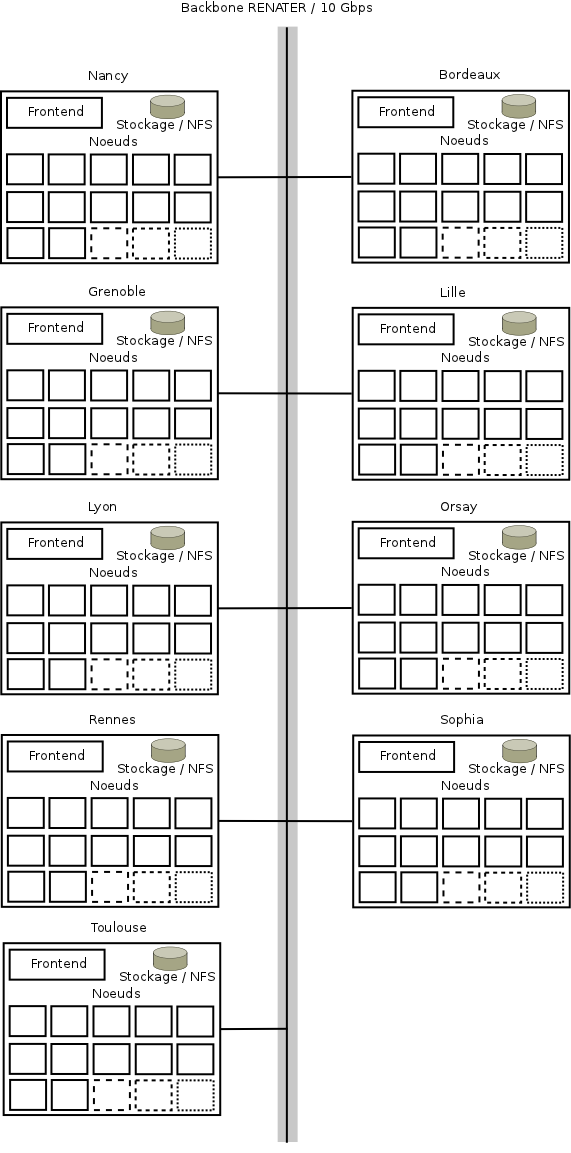
\includegraphics[width=10cm,height=15cm]{images/g5k1.png}
\\
\underline{\textit{Architecture Grid5000}}
%%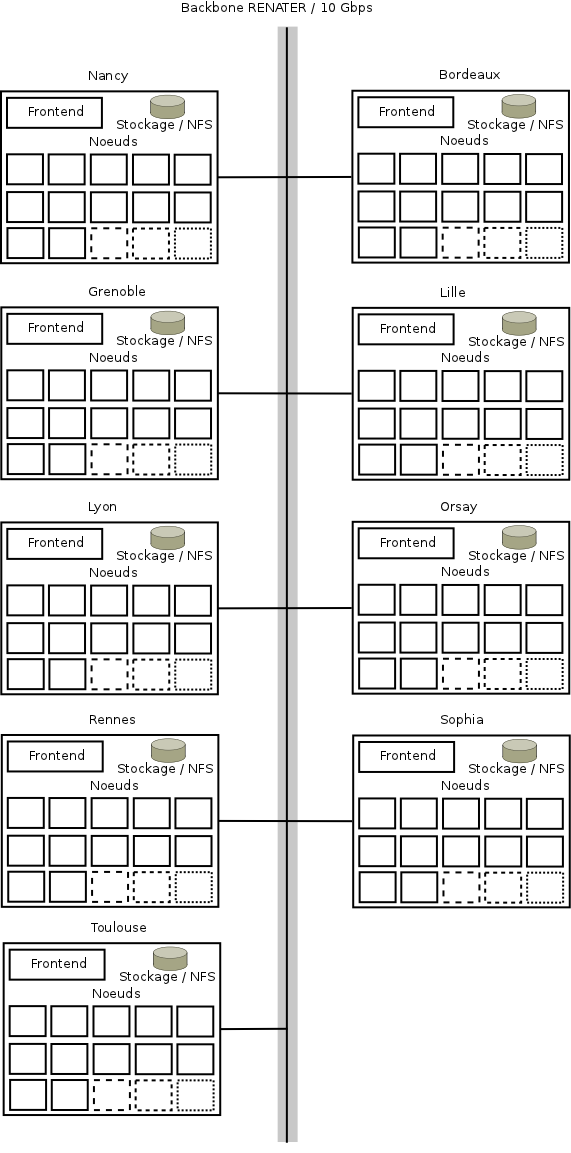
\includegraphics{images/g5k1.png}
\end{center}
L'utilisateur de Grid 5000 accède à chaque site par son frontend en utilisant le protocole SSH.\\
Commande:
\begin{lstlisting}
ssh utilisateur@access.grid5000.fr
\end{lstlisting}
Sur tous les serveurs du site, un répertoire home, local à chaque site, est monté avec NFS 2 .
A partir du frontend, il est possible d'accéder aux machines des clusters en exectuant des réservations à l'aide de la commande:
\begin{lstlisting}
oarsub
\end{lstlisting}
Gràce à notre tuteur, M. Lucas Nussbaum nous avons pu visiter la salle serveurs du site de Nancy située au Loria, 
ainsi qu'une présentation de la plate-forme (matériel utilisé, connexions réseau,
administration).
\quotation\textit{Une description détaillée du site de Nancy est disponible sur le site de Grid 5000.}

  \subsection{Réseau}
Les sites et toutes les machines qu'ils comprennent sont interconnectés par RENATER 3 en 10Gbits/s. De
plus, chaque site peut disposer de plusieurs réseaux locaux 4 :
\begin{itemize}
\item réseau en ethernet, 1 Gb/s
\item réseaux hautes performances (Infiniband 20 Gb/s ou 10 Gb/s, et Myrinet 20 Gb/s)
\end{itemize}

  \subsection{Environnement logiciel}
Tous les serveurs de Grid 5000 fonctionnent sous Debian GNU/Linux.
A partir du frontend, l'utilisateur peut réserver des machines en utilisant la suite de logiciels OAR dédiée à
la gestion de ressources de clusters, et déployer ses propres images de systèmes à l'aide des outils kadeploy.
Il y a deux types de réservation :
\begin{itemize}
\item par défaut, pour des besoins de calcul avec OpenMPI ;
\item pour le déploiement d'environnements (deploy ).
\end{itemize}


\section{Répartition des tâches}
Nous avons commencé par prendre en main Grid5000 durant les 2 premières semaines du projet. Pour ce faire nous avons suivi avec soin les tutoriels mis à notre disposition sur le site www.grid5000.fr.

Une fois les manipulations de bases bien assimilées. Nous nous sommes divisés en 2 sous-groupes pour tester les différents outils du projet :
\begin{itemize}
  \item Julien et Augustin se sont chargés de Ganeti et archipel.
  \item Sébatien et Mathieu pour OpenXenManager et virt-manager.
\end{itemize}


\chapter{Ganeti}
\section{Introduction}
Ganeti est un outil de gestion de machines virtuelles se basant sur les technologies de virtualisation existantes comme XEN et KVM.\\
<<<<<<< HEAD
Ganeti n�cessite un logiciel de virtualisation pr�-install� sur les serveurs afin de pouvoir fonctionner. Une fois install�, 
l'outil prendra en charge la partie gestion des instances virtuelles (Xen DomU), par exemple, la gestion de cr�ation de disque, 
l'installation du syst�me d'exploitation (en coop�ration avec les scripts d'installation du syst�me d'exploitation 
sp�cifique), et le d�marrage, l'arr�t, le basculement entre les syst�mes physiques. Il a �t� con�u pour faciliter la gestion de 
cluster de serveurs virtuels et de fournir une r�cup�ration rapide et simple.


\section {Installation}
\subsection {Modification des sources}
Nous avons intall� ganeti � partir de la branche testing de debian. Pour des raisons techniques le syst�me est squeeze. Pour cela il faut ajouter les sources de testing dans le fichier /etc/apt/sources.list :
=======
%Ganeti nécessite un logiciel de virtualisation pré-installé sur les serveurs afin de pouvoir fonctionner. Une fois installé, l'outil prendra en charge la partie gestion des instances virtuelles (Xen DomU), par exemple, la gestion de création de disque, l'installation du système d'exploitation (en coopération avec les scripts d'installation du système d'exploitation spécifique), et le démarrage, l'arrêt, le basculement entre les systèmes physiques. Il a été conçu pour faciliter la gestion de cluster de serveurs virtuels et de fournir une récupération rapide et simple.

\section{Installation}
\subsection{Modification des sources}
Nous avons intallé ganeti à partir de la branche testing de debian. Pour des raisons techniques le système est squeeze. Pour cela il faut ajouter les sources de testing dans le fichier /etc/apt/sources.list :
>>>>>>> bdb35216a929de37c6411ee8791b131964b0fad8
\begin{lstlisting}
##Wheezy
deb http://ftp.fr.debian.org/debian/ wheezy main contrib non-free
deb-src http://ftp.fr.debian.org/debian/ wheezy main contrib non-free

## wheezy security
deb http://security.debian.org/ wheezy/updates main contrib non-free
deb-src http://security.debian.org/ wheezy/updates main contrib non-free
\end{lstlisting}

IL faut ensuite cr�er le fichier de pr�f�rence de apt dans le r�pertoire /etc/apt/apt.conf.d. Nous avons appel� le  fichier 80default-distrib (le nom du fichier est libre). Il faut ajouter cette ligne au fichier qui d�fini la branche stable comme la branche par d�faut :
\begin{lstlisting}
APT::Default-Release "stable";
\end{lstlisting}

<<<<<<< HEAD
\subsection {Mise � jour et installation}
On peut enfin alors mettre le syst�me � jour et installer ganeti :
=======
\subsection{Mise à jour et installation}
On peut enfin alors mettre le système à jour et installer ganeti :
>>>>>>> bdb35216a929de37c6411ee8791b131964b0fad8

\begin{lstlisting}
apt-get update && apt-get dist-upgrade -q -y --force-yes
apt-get -t testing install -q -y --force-yes ganeti2 ganeti-htools ganeti-instance-debootstrap
\end{lstlisting}

\section{Configuration}

La configuration est l'�tape la plus complexe.

\subsection{Configuration du fichier hosts}

Dans le fichier hosts il faut renseigner l'adresse et le nom complet du node primaire de cette mani�re :
\begin{lstlisting}
172.16.68.10    griffon-10.nancy.grid5000.fr griffon-10
\end{lstlisting}
\subsection{Copie de vmlinuz-2.6.32-5-xen-amd64 et initrd.img-2.6.32-5-xen-amd64}
Dans /etc/boot copier les fichiers vmlinuz-2.6.32-5-xen-amd64 et initrd.img-2.6.32-5-xen-amd64 :
\begin{lstlisting}
cp vmlinuz-2.6.32-5-xen-amd64 vmlinuz-2.6-xenU
cp initrd.img-2.6.32-5-xen-amd64 initrd.img-2.6-xenU
\end{lstlisting}

<<<<<<< HEAD
\subsection {Cr�ation du bridge xen-br0}

\subsection {Cr�ation du LVM}
=======
\subsection{Création du bridge xen-br0}
BLABLABLA
\subsection{Création du LVM}
>>>>>>> bdb35216a929de37c6411ee8791b131964b0fad8

Ganeti requi�re un LVM d'au moins 20Go pour fonctionner.

Sur les neud de grid5000 il est possible de cr�er un tel LVM sur la partition /dev/sd5.
\begin{lstlisting}
umount /dev/sda5
pvcreate /dev/sda5
vgcreate xenvg /dev/sda5
\end{lstlisting}
On a cr�� un VG qui se nome xenvg sur /dev/sda5.

\subsection{Edition de /usr/share/ganeti/os/debootstrap/common.sh}

Il est n�cessaire d'�diter ce fichier pour que ganeti puisse cr�er des instances :

<<<<<<< HEAD
Par defaut le mirroir utilis� par ganeti est http://ftp.us.debian.org/debian/. Sur Grid5000 les depots US sont bloqu�s. Il faut donc indiquer les depots francais.
On indique aussi l'adresse du  proxy de grid5000.
On peut choisir la version de Debian que l'on souhaite installer. Ici nous avons opter pour squeeze.
L'architecture que nous choisi est amd64, car l'hote la supporte.
La variable : extra_pkdg permet d'installer des paquets suppl�mentaires.
=======
%Par défaut le mirroir utilisé par ganeti est http://ftp.us.debian.org/debian/. Sur Grid5000 les depots US sont bloqués. Il faut donc indiquer les depots francais. On indique aussi l'adresse du  proxy de grid5000. On peut choisir la version de Debian que l'on souhaite installer. Ici nous avons opter pour squeeze. L'architecture que nous choisi est amd64, car l'hôte la supporte. La variable : EXTRA_PKGS permet d'installer des paquets supplémentaires.
>>>>>>> bdb35216a929de37c6411ee8791b131964b0fad8

\subsection{Configuration et initialisation du cluster}
L'initialisation du cluster se fait avec la commande gnt-cluster init clusterX
\begin{lstlisting}
#initialisation du cluster
gnt-cluster init --no-drbd-storage --nic-parameters link=eth0 cluster1
\end{lstlisting}
Ici nous avons pr�cis� les options --no-drbd-storage --nic-parameters link=eth0.
La premi�re permet d'utiliser ganeti sans utiliser la haute disponibilit�.
La seconde permet de pr�ciser un autre bridge que xen-br0

Enfin il faut renseigner le inird et le root_path, cela est n�cessaire pour la cr�ation des instances :
\begin{lstlisting}
gnt-cluster modify --hypervisor-parameter xen-pvm:initrd_path='/boot/initrd.img-2.6-xenU'
gnt-cluster modify --hypervisor-parameter xen-pvm:root_path='/dev/xvda1'
\end{lstlisting}  
<<<<<<< HEAD

\section {Utilisation des nodes}
\subsection {Ajouter un node}
Il est possible d'ajouter un node  tout moment :
=======
\section{Utilisation des nodes}
\subsection{Ajouter un node}
Il est possible d'ajouter un node à tout moment :
>>>>>>> bdb35216a929de37c6411ee8791b131964b0fad8
\begin{lstlisting}
root@griffon-8: gnt-node add griffon-78.nancy.grid5000.fr

-- WARNING -- 
Performing this operation is going to replace the ssh daemon keypair
on the target machine (griffon-78.nancy.grid5000.fr) with the ones of the current one
and grant full intra-cluster ssh root access to/from it

Unable to verify hostkey of host griffon-78.nancy.grid5000.fr:
30:cb:8f:ec:16:6a:3b:f5:0c:2a:de:a6:4c:1d:00:19. Do you want to accept
it?
y/[n]/?: y
2012-03-12 07:38:09,239: MainThread Authentication to griffon-78.nancy.grid5000.fr via public key failed, trying password
root password:
Mon Mar 12 07:38:16 2012  - INFO: Node will be a master candidate
\end{lstlisting}
\subsection{Reconfigurer un node}
Il aussi possible de reconfigurer un node deja pr�sent :
\begin{lstlisting}
root@griffon-8: gnt-node add --readd griffon-78.nancy.grid5000.fr

Unable to verify hostkey of host griffon-78.nancy.grid5000.fr:
6c:10:44:28:e2:2c:fc:7f:d4:5e:a3:bd:83:2c:b2:97. Do you want to accept
it?
y/[n]/?: y
Mon Mar 12 07:39:36 2012  - INFO: Readding a node, the offline/drained flags were reset
Mon Mar 12 07:39:36 2012  - INFO: Node will be a master candidate
\end{lstlisting}
\subsection{Changer les roles des nodes}

\subsubsection {Promouvoir un neud au rang de master :}
%Il faut d'abord revoquer le rang de master du node principal, sur un node master-candidate :
\begin{lstlisting}
gnt-cluster master-failover

root@griffon-81: gnt-instance list
Failure: prerequisites not met for this operation:
This is not the master node, please connect to node 'griffon-8.nancy.grid5000.fr' and rerun the command

root@griffon-81: gnt-cluster master-failover

root@griffon-81: gnt-node list
Node                         DTotal  DFree MTotal MNode MFree Pinst Sinst
griffon-8.nancy.grid5000.fr  283.2G 283.2G  16.0G  965M 14.8G     0     0
griffon-78.nancy.grid5000.fr 283.2G 283.2G  16.0G  965M 14.8G     0     0
griffon-81.nancy.grid5000.fr 283.2G 283.2G  16.0G  965M 14.8G     0     0
\end{lstlisting}
<<<<<<< HEAD
On voit que le node griffon-81 n'�tait pas master avant l'utilisation de la commande. Ensuite il est possible d'executer les commandes master.
=======
%On voit que le node griffon-81 n'était pas master avant l'utilisation de la commande. Ensuite il est possible d'executer les commandes master.
>>>>>>> bdb35216a929de37c6411ee8791b131964b0fad8

\subsubsection{Passer un neud en master-candidate :}
\begin{lstlisting}
root@griffon-81: gnt-node modify -C yes griffon-8.nancy.grid5000.fr
Modified node griffon-8.nancy.grid5000.fr
 - master_candidate -> True
 - drained -> False
\end{lstlisting}
\subsubsection{Passer un node en status drained :}
\begin{lstlisting}
root@griffon-81: gnt-node modify -D yes griffon-8.nancy.grid5000.fr
Modified node griffon-8.nancy.grid5000.fr
 - master_candidate -> False
 - drained -> True
\end{lstlisting}
\subsubsection{Passer un node en offline :}
\begin{lstlisting}
root@griffon-81: gnt-node modify -O yes griffon-8.nancy.grid5000.fr
Modified node griffon-8.nancy.grid5000.fr
 - master_candidate -> False
 - offline -> True
\end{lstlisting}
<<<<<<< HEAD
\subsubsection {Passer un node en mode regular (remise � zero de tous les flags) :}
=======
\subsubsection{Passer un node en mode regular (remise à zero de tous les flags) :}
>>>>>>> bdb35216a929de37c6411ee8791b131964b0fad8
\begin{lstlisting}
root@griffon-81: gnt-node modify -O no -D no -C no griffon-8.nancy.grid5000.fr
Mon Mar 12 08:26:01 2012  - INFO: Ignoring request to unset flag master_candidate, already unset
Mon Mar 12 08:26:01 2012  - INFO: Ignoring request to unset flag drained, already unset
Mon Mar 12 08:26:01 2012  - INFO: Auto-promoting node to master candidate
Mon Mar 12 08:26:01 2012  - WARNING: Transitioning node from offline to online state without using re-add. Please make sure the node is healthy!
Modified node griffon-8.nancy.grid5000.fr
 - master_candidate -> True
 - offline -> False
\end{lstlisting}
Le node est de nouveau en master-candidate comme � l'origine.

\subsection{Supprimer un node :}
\begin{lstlisting}
root@griffon-81: gnt-node list
Node                         DTotal  DFree MTotal MNode MFree Pinst Sinst
griffon-8.nancy.grid5000.fr  283.2G 282.2G  16.0G  965M 14.7G     1     0
griffon-78.nancy.grid5000.fr 283.2G 283.2G  16.0G  965M 14.8G     0     0
griffon-81.nancy.grid5000.fr 283.2G 283.2G  16.0G  965M 14.8G     0     0

root@griffon-81: gnt-node remove griffon-78.nancy.grid5000.fr

root@griffon-81: gnt-node list
Node                         DTotal  DFree MTotal MNode MFree Pinst Sinst
griffon-8.nancy.grid5000.fr  283.2G 282.2G  16.0G  965M 14.7G     1     0
griffon-81.nancy.grid5000.fr 283.2G 283.2G  16.0G  965M 14.8G     0     0
\end{lstlisting}
Le node griffon-78 � bien �t� effacer du cluster.

\subsection{Manipulation du stockage :}

Faire la liste des volumes sur lesquels sont les instances : 
\begin{lstlisting}
root@griffon-81: gnt-node volumes
Node                         PhysDev   VG    Name                                        Size Instance 
griffon-81.nancy.grid5000.fr /dev/sda5 xenvg 4b328fb6-1cc9-4599-9523-2c6a8cf7b861.disk0 1000M instance4
griffon-8.nancy.grid5000.fr  /dev/sda5 xenvg 8a85c87b-39fa-4e88-886b-a60c8706cc65.disk0 1000M instance2
griffon-8.nancy.grid5000.fr  /dev/sda5 xenvg d84f3842-04d5-4951-aded-b5ea76f19681.disk0 1000M instance1
griffon-8.nancy.grid5000.fr  /dev/sda5 xenvg ddfea3fc-d7b1-4a06-ae37-3094b1f0de11.disk0 1000M instance3
\end{lstlisting}
Il est possible de lancer une reparation sur les volume de stockage :
\begin{lstlisting}
root@griffon-81:~# gnt-node repair-storage griffon-8.nancy.grid5000.fr lvm-vg xenvg
Mon Mar 12 09:56:23 2012 Repairing storage unit 'xenvg' on griffon-8.nancy.grid5000.fr ...
\end{lstlisting}
Cela �quivau � vgreduce --removemissing.



\section{Utilisation des instances}

\subsection{Ajouter une instance}
\begin{lstlisting}
root@graphene-11: gnt-instance add -n graphene-11.nancy.grid5000.fr -o debootstrap+default -t plain -s 1000 instance1

Sat Mar 10 16:52:35 2012 * disk 0, vg xenvg, name 99370e22-9421-40d6-8d9d-59bb6ecfa959.disk0
Sat Mar 10 16:52:35 2012 * creating instance disks...
Sat Mar 10 16:52:36 2012 adding instance instance1 to cluster config
Sat Mar 10 16:52:36 2012  - INFO: Waiting for instance instance1 to sync disks.
Sat Mar 10 16:52:37 2012  - INFO: Instance instance1's disks are in sync.
Sat Mar 10 16:52:37 2012 * running the instance OS create scripts...
Sat Mar 10 16:54:05 2012 * starting instance...

root@graphene-11: gnt-instance list
Instance  Hypervisor OS                  Primary_node                  Status  Memory
instance1 xen-pvm    debootstrap+default graphene-11.nancy.grid5000.fr running   128M
\end{lstlisting}
L'instance est bien cr�er sur le neud. Il est possible � partir du maitre de cr�er des instances sur n'importe quels neud d'un cluster. Il aussi possible de cr�er une instance primaire sur un noeud et une instance secondaire sur un autre.

\subsection{Supprimer une instance}
\begin{lstlisting}
root@graphene-11: gnt-instance remove instance1
This will remove the volumes of the instance instance1 (including
mirrors), thus removing all the data of the instance. Continue?
y/[n]/?: y

root@graphene-11: gnt-instance list
Instance Hypervisor OS Primary_node Status Memory
\end{lstlisting}
L'instance � bien �t� supprim�e. Cette commande supprime l'instance quelque soit le ou les neud o� elle a �t� cr�er.


Arret et demarrage d'une instance
\begin{lstlisting}
root@graphene-11: gnt-instance list
Instance  Hypervisor OS                  Primary_node                  Status  Memory
instance1 xen-pvm    debootstrap+default graphene-11.nancy.grid5000.fr running   128M
instance2 xen-pvm    debootstrap+default graphene-11.nancy.grid5000.fr running   128M

root@graphene-11: gnt-instance shutdown instance2
Waiting for job 21 for instance2...

root@graphene-11: gnt-instance list
Instance  Hypervisor OS                  Primary_node                  Status     Memory
instance1 xen-pvm    debootstrap+default graphene-11.nancy.grid5000.fr running      128M
instance2 xen-pvm    debootstrap+default graphene-11.nancy.grid5000.fr ADMIN_down      -
\end{lstlisting}


\begin{lstlisting}
root@graphene-11: gnt-instance startup instance2
Waiting for job 26 for instance2...

root@graphene-11: gnt-instance list
Instance  Hypervisor OS                  Primary_node                  Status  Memory
instance1 xen-pvm    debootstrap+default graphene-11.nancy.grid5000.fr running   128M
instance2 xen-pvm    debootstrap+default graphene-11.nancy.grid5000.fr running   128M
\end{lstlisting}
Le status de instance2 est de nouveau "running" ce qui signifie qu'elle est en fonctionnement.

Interroger les instances :
\begin{lstlisting}
root@graphene-11: gnt-instance info instance1

Instance name: instance1
UUID: 3c3bd5ac-a261-4cba-a7f3-6cc74e49ce4e
Serial number: 2
Creation time: 2012-03-10 17:06:56
Modification time: 2012-03-10 17:07:04
State: configured to be up, actual state is up
  Nodes:
    - primary: graphene-11.nancy.grid5000.fr
    - secondaries: 
  Operating system: debootstrap+default
  Allocated network port: None
  Hypervisor: xen-pvm
    - blockdev_prefix: default (sd)
    - bootloader_args: default ()
    - bootloader_path: default ()
    - initrd_path: default (/boot/initrd.img-2.6-xenU)
    - kernel_args: default (ro)
    - kernel_path: default (/boot/vmlinuz-2.6-xenU)
    - root_path: default (/dev/sda1)
    - use_bootloader: default (False)
  Hardware:
    - VCPUs: 1
    - memory: 128MiB
    - NICs:
      - nic/0: MAC: aa:00:00:d8:c6:8a, IP: None, mode: bridged, link: xen-br0
  Disk template: plain
  Disks:
    - disk/0: lvm, size 1000M
      access mode: rw
      logical_id:  xenvg/3fe11555-edcd-40dc-bf63-f3fb749825bb.disk0
      on primary:  /dev/xenvg/3fe11555-edcd-40dc-bf63-f3fb749825bb.disk0 (254:0)
\end{lstlisting}
Cette commande �dite les informations relatives � l'instance.


Import et export d'instances :

Export :
\begin{lstlisting}
root@graphene-100: gnt-backup export -n graphene-143.nancy.grid5000.fr instance1
Sun Mar 11 14:06:04 2012 Shutting down instance instance1
Sun Mar 11 14:08:07 2012 Creating a snapshot of disk/0 on node graphene-100.nancy.grid5000.fr
Sun Mar 11 14:08:08 2012 Starting instance instance1
Sun Mar 11 14:08:09 2012 Exporting snapshot/0 from graphene-100.nancy.grid5000.fr to graphene-143.nancy.grid5000.fr
Sun Mar 11 14:08:13 2012 snapshot/0 is now listening, starting export
Sun Mar 11 14:08:17 2012 snapshot/0 is receiving data on graphene-143.nancy.grid5000.fr
Sun Mar 11 14:08:17 2012 snapshot/0 is sending data on graphene-100.nancy.grid5000.fr
Sun Mar 11 14:08:22 2012 snapshot/0 sent 14M, 2.8 MiB/s
Sun Mar 11 14:08:38 2012 snapshot/0 finished receiving data
Sun Mar 11 14:08:38 2012 snapshot/0 finished sending data
Sun Mar 11 14:08:38 2012 Removing snapshot of disk/0 on node graphene-100.nancy.grid5000.fr
Sun Mar 11 14:08:39 2012 Finalizing export on graphene-143.nancy.grid5000.fr
Sun Mar 11 14:08:40 2012 Removing old exports for instance instance1
\end{lstlisting}
L'instance � bien �t� export� dans graphene-143.nancy.grid5000.fr

Il est tout � fait possible d'exporter une instance sans la red�marer en utilisant l'option : --noshutdown.

Import :
\begin{lstlisting}
root@graphene-100: gnt-instance remove instance1
This will remove the volumes of the instance instance1 (including
mirrors), thus removing all the data of the instance. Continue?
y/[n]/?: y

root@graphene-100: gnt-instance list
Instance  Hypervisor OS                  Primary_node                   Status  Memory
instance2 xen-pvm    debootstrap+default graphene-100.nancy.grid5000.fr running   128M
instance3 xen-pvm    debootstrap+default graphene-143.nancy.grid5000.fr running   128M
\end{lstlisting}
Instance1 � �t� supprim�e du cluster.
\begin{lstlisting}
root@graphene-100: gnt-backup import -n graphene-100.nancy.grid5000.fr --src-node=graphene-143.nancy.grid5000.fr -t plain instance1
Sun Mar 11 14:22:29 2012 * disk 0, vg xenvg, name a4cc7447-5ed7-4417-b222-d33a0c2842a0.disk0
Sun Mar 11 14:22:29 2012 * creating instance disks...
Sun Mar 11 14:22:30 2012 adding instance instance1 to cluster config
Sun Mar 11 14:22:30 2012  - INFO: Waiting for instance instance1 to sync disks.
Sun Mar 11 14:22:30 2012  - INFO: Instance instance1's disks are in sync.
Sun Mar 11 14:22:30 2012 * running the instance OS import scripts...
Sun Mar 11 14:22:30 2012 Exporting disk/0 from graphene-143.nancy.grid5000.fr to graphene-100.nancy.grid5000.fr
Sun Mar 11 14:22:34 2012 disk/0 is now listening, starting export
Sun Mar 11 14:22:37 2012 disk/0 is receiving data on graphene-100.nancy.grid5000.fr
Sun Mar 11 14:22:37 2012 disk/0 is sending data on graphene-143.nancy.grid5000.fr
Sun Mar 11 14:22:42 2012 disk/0 sent 34M, 6.0 MiB/s, 19%, ETA 23s
Sun Mar 11 14:23:08 2012 disk/0 finished sending data
Sun Mar 11 14:23:14 2012 disk/0 finished receiving data
\end{lstlisting}
On importe instance1 depuis graphene-143.nancy.grid5000.fr.
\begin{lstlisting}
root@graphene-100: gnt-instance list
Instance  Hypervisor OS                  Primary_node                   Status     Memory
instance1 xen-pvm    debootstrap+default graphene-100.nancy.grid5000.fr ADMIN_down      -
instance2 xen-pvm    debootstrap+default graphene-100.nancy.grid5000.fr running      128M
instance3 xen-pvm    debootstrap+default graphene-143.nancy.grid5000.fr running      128M
\end{lstlisting}
L'instance � bien �t� import�e.
\begin{lstlisting}
root@graphene-100: gnt-instance startup instance1
Waiting for job 32 for instance1...

root@graphene-100: gnt-instance list
Instance  Hypervisor OS                  Primary_node                   Status  Memory
instance1 xen-pvm    debootstrap+default graphene-100.nancy.grid5000.fr running   128M
instance2 xen-pvm    debootstrap+default graphene-100.nancy.grid5000.fr running   128M
instance3 xen-pvm    debootstrap+default graphene-143.nancy.grid5000.fr running   128M
\end{lstlisting}
L'instance est fonctionnelle sur graphene-100.nancy.grid5000.fr


IL est aussi possible d'importer une instance �trang�re � ganeti dont le disque est deja dans un LVM, sans avoir � le recopier.

\begin{lstlisting}
gnt-instance add -t plain -n HOME_NODE ... \
  --disk 0:adopt=lv_name[,vg=vg_name] INSTANCE_NAME
\end{lstlisting}

Connexion � la console d'un instance :
\begin{lstlisting}
gnt-instance console instance5
\end{lstlisting}

\lstset{language=bash}
\chapter{OpenXENManager}
\section{Présentation}
XenseMaking Project développe un client lourd, ainsi qu'un client
web, pour manager XenServer. C'est un clone du XenCenter, qui fonctionne
avec Linux, BSD, Windows et MacOSX, alors que le XenCenter ne fonctionne
qu'avec Windows. OpenXenManager/OpenXenCenter un le client lourd qui
permet de manager XenServer.Il a été développé en Python avec pygtk
et gtk-vnc.
Les fonctionnalités actuellement implémentées sont les suivantes :
\begin{itemize}
\item monitoring des machines virtuelles - accès à la console des machines virtuelles
\item opérations d'administration (démarrage, arrèt, reboot, ...)
\item création de machines virtuelles
\end{itemize}
\section{Installation}
Pour l'installation nous avons besoin des paquets suivant:
\begin{lstlisting}
apt-get install subversion bzip2 python-glade2 python-gtk-vnc shared-mime-info graphviz
\end{lstlisting}
On télécharge la dernière version d'openxenmanager dans le dépot subversion
\begin{lstlisting}
svn co https://openxenmanager.svn.sourceforge.net/svnroot/openxenmanager openxenmanager
\end{lstlisting}
On se déplace dans le répertoire trunk:
\begin{lstlisting}
cd openxenmanager/trunk
\end{lstlisting}
Finalement on lance openxenmanager avec la commande suivante
\begin{lstlisting}
python window.py
\end{lstlisting}
Une interface graphique d'openxenmanger apparait.
\section{Utilisation}
Pour l'instant nous n'avons toujours pas réussi à utiliser ce logiciel. DU a diverses difficultées (pas de service distant sous squeeze et plus de xen lors de la migration sous unstable).

\chapter{Virt-manager}
\section{Pré-requis et considérations pour les hôtes}
Divers facteurs doivent être considérés avant de créer des hôtes virtualisés.
\subsubsection{Performance} 
Les hôtes virtualisés doivent être déployé et configuré en fonction de leurs tâches prévues. Certains systèmes (par exemple, les hôtes ou sont hébergés des serveur de base de données) ont besoin de performances plus élevées que d'habitude; Les hôtes peuvent exiger plus de CPU ou de mémoire attribué en fonction de leur rôle,et de l'utilisation futur qu'il pourrait avoir. projeté la charge du système.
\subsubsection{Stockage}
Certains hôtes peuvent avoir besoin d'une plus grande priorité d'accès au stockage, de disques plus rapides, ou peuvent exiger un accès exclusif à des zones de stockage. La quantité de stockage utilisée par les hôtes doit être régulièrement surveillée et prise en compte lors du déploiement et le maintien de stockage.
\subsubsection{Mise en réseau et l'infrastructure du réseau}
 En fonction de notre environnement, certains hôtes pourraient exiger des liens réseau plus rapides que d'autres hôtes. La bande passante ou de latence sont souvent des facteurs à prendre en compte lors du déploiement et le maintenance des hôtes.
\section{Installation côté serveur}
Cette partie est facile, un simple apt-get install suffit. Nous installons le paquet qui communique avec Xen et remonte les informations au client virt-manager.
\begin{lstlisting}
apt-get install libvirt-bin
\end{lstlisting} 
Du coté de Xen, nous devons vérifier qu’il peut communiquer avec libvirt.

Libvirt accède aux données de Xen via un socket unix. La configuration consiste à activer cette option dans Xen et à relancer les services.
Nous éviterons ainsi l’erreur \emph{libvirtError: internal error failed to connect to xend} dont on trouve peu d’explication sur le net.
\\
Un autre bug rencontré nécessite la correction d'un lien symbolique et l'installation de qemu.

\begin{lstlisting}
# Installation de qemu-dm pour créer des machines virtuelles en mode full virtualisé
apt-get install xen-qemu-dm-4.0 -y

# Correction d'un bug de qemu qui invalidait un lien symbolique
mkdir /usr/lib64/xen
mkdir /usr/lib64/xen/bin
cd /usr/lib64/xen/bin
ln -s /usr/lib/xen-4.0/bin/qemu-dm
\end{lstlisting} 

On édite le fichier de configuration xen
\begin{lstlisting} 
nano /etc/xen/xend-config.sxp
\end{lstlisting}
 on active la ligne suivante
\begin{lstlisting} 
(xend-unix-server yes)
\end{lstlisting}
 Enfin on relance le service xen avec /etc/init.d/xend restart

\section{Installation côté client}
Pour gérer nos serveurs, nous installons virt-manager avec la commande suivante:
\begin{lstlisting} 
apt-get install virt-manager
\end{lstlisting}
Virt-manager étant un outil graphique, ses fichiers de configurations sont gérés par gconf. Ainsi, pour automatiser l'ajout des différents noeuds nous avons crée un script qui réécrit le fichier \emph{~/.gconf/apps/virt-manager/connections/\%gconf.xml}
\begin{lstlisting}
for node in $(cat $list_nodes)
do
    echo '<li type="string">' >> $fichier
    echo "<stringvalue>xen+ssh://root@$node/</stringvalue>" >> $fichier
    echo '</li>' >> $fichier
done
\end{lstlisting}
Ce fichier est au format xml et contient pour chaque noeud une entrée. Ici, les connexions sont gérées au-dessus d'un tunnel ssh.
\section{Création d'hôtes virtualisés avec virt-manager}
1)Pour commencer on démarre virt-manager, puis on lance le gestionnaire de machines virtuelles à partir du menu en cliquant sur l'icone en forme de pc.

%\begin{figure}
\begin{center}
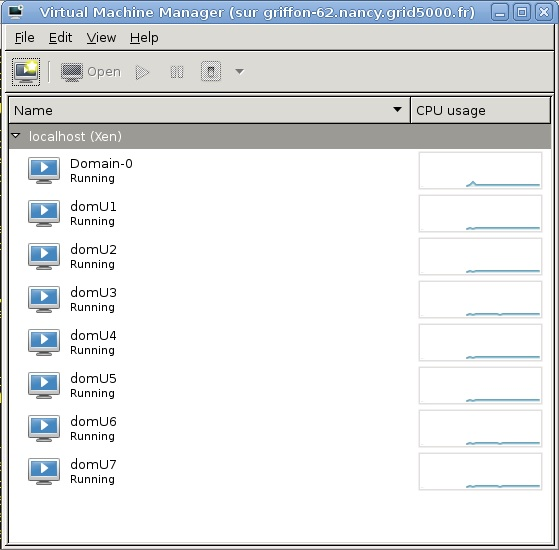
\includegraphics[width=350pt]{images/virt.jpg}
\end{center}
%\caption{Interface de virt-manager}
%\end{figure}

3) La fenêtre du gestionnaire de machine virtuelle nous autorise à en créer de nouvelles.
On clique sur création de nouvelle machine virtuelle pour faire apparaître l'assistant qui va nous aider pour élaborer notre hôte.
L'assistant décompose la création en cinq étapes:
-La localisation et la configuration des supports d'installation
-La configuration de la mémoire et les options de CPU
-La configuration du stockage de l'invité
-La configuration réseau, l'architecture, et d'autres paramètres matériels

Le processus de création d'hôte commence avec la selection d'un nom et le type d'installation.
%\begin{figure}
\begin{center}
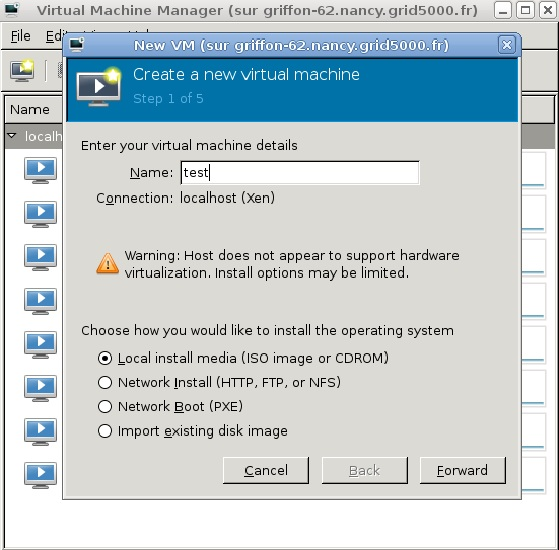
\includegraphics[width=350pt]{images/nommachine.jpg}
\end{center}
%\caption{Choix du nom de la nouvelle machine virtuelle}
%\end{figure}
-Local install media(ISO image or CDROM)
Cette méthode utilise un CD-ROM,DVD ou une image iso.

-Network install
Cette méthode utilise le réseau pour installer le système d'exploitation.

-Import existing disk image
Cette méthode nous permet de créer un nouvelle hôte et d'y importer une image disque.

La prochaine étape consiste à configurer l'installation.
On configure le type de système d'exploitation et sa version qui sera installé, cela dépend de la méthode d'installation que l'on a choisie.
%\begin{figure}
\begin{center}
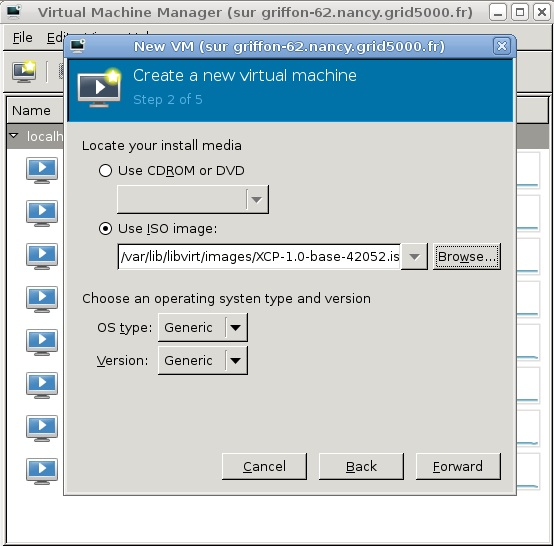
\includegraphics[width=300pt]{images/iso.jpg}
\end{center}
%\caption{Choix du nom de la nouvelle machine virtuelle}
%\end{figure}

Configuration du CPU et de la mémoire
La prochaine étape consiste à configurer le nombre de CPU et la quantité de mémoire à allouer à la machine virtuelle. L'assistant indique le nombre de processeurs et la quantité de mémoire que l'on peut lui allouer.
%\begin{figure}
\begin{center}
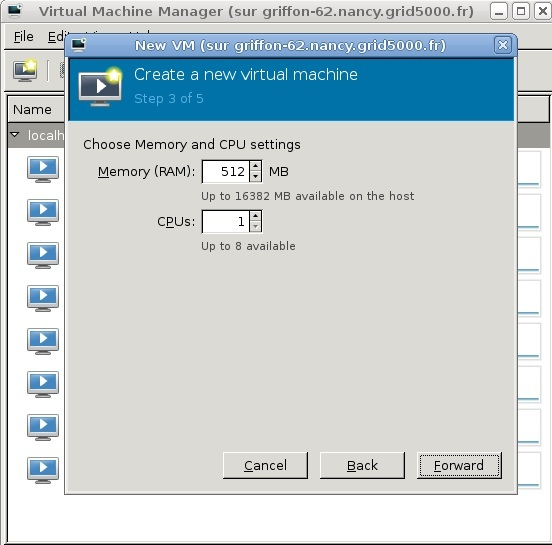
\includegraphics[width=300pt]{images/cpu.jpg}
\end{center}
%\caption{Configuration du CPU et de la mémoire allouée à la machine virtuelle}
%\end{figure}

Configuration de l'espace de stockage
%\begin{figure}
\begin{center}
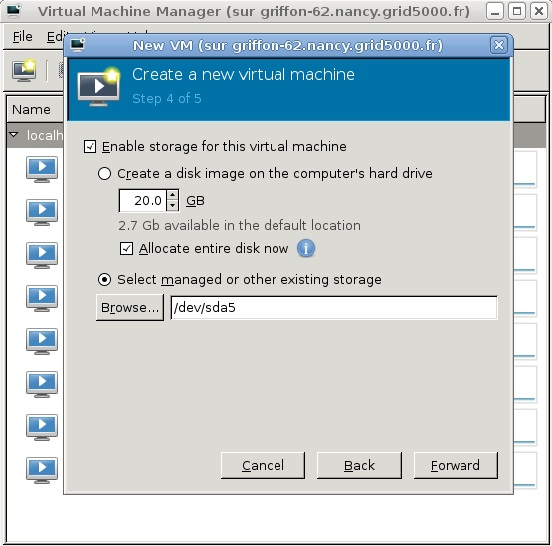
\includegraphics[width=300pt]{images/Storage.jpg}
\end{center}
%\caption{Choix du stockage de la machine virtuelle}
%\end{figure}

 Si l'on a choisi d'importer une image de disque existante au cours de la première étape, virt-manager va sauter cette étape.
On doit attribuer un espace suffisant pour notre machine virtuelle et toutes les applications que l'hôte a besoin.

Configuration finale
On vérifie les paramètres de la machine virtuelle et on clique sur Terminer lorsqu'on est satisfait, cela permettra de créer l'hôte avec les paramètres réseau par défaut, le type de virtualisation, et l'architecture.
\begin{center}
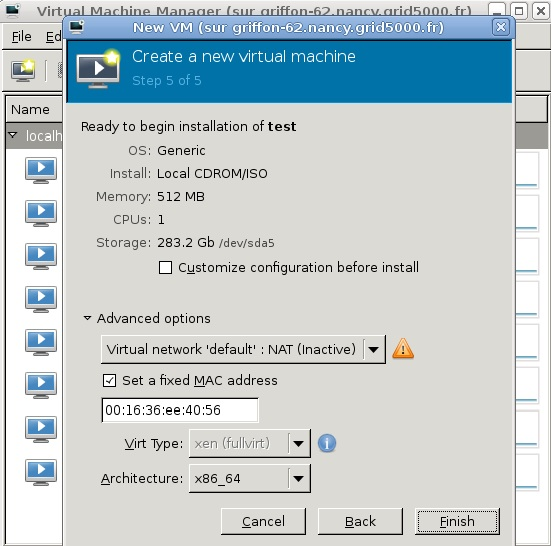
\includegraphics[width=300pt]{images/reseau.jpg}
\end{center}
%\caption{Configuration du réseau}


\subsection{Controle d'hotes distants}
On peut facilement manager des hotes distants une fois ceux-ci enregistrés dans virt-manager. Cette opération peut être fastidieuse car virt étant un programme graphique, crée un script pour automatiser l'ajout de plusieurs dizaines de noeuds s'est avéré plus compliqué que prévu.
Cherchant désespérément un fichier de configuration, nous avons fini par le trouver en lançant une recherche dans tout le système sur les noms des noeuds ajoutés à virt. Le fichier est donc géré par \emph{gconf} en voici un exemple
\lstinputlisting[language=xml,morekeywords={li,entry,stringvalue,gconf}]{scripts/virt-manager/gconf.xml}
Après l'installation de virt, le seul lien enregistré est le lien local. Pour ajouter une connexion vers un nouvel hote xen, on peut utiliser l'interface graphique.
%\includegraphics image ajout d'un noeud
Cependant, dans notre cas, il était assez fastidieux de renseigner manuellelement chacun des noeuds surtout lors des tests à grande échelle. C'est pourquoi nous avons fait un script (voir annexe \ref{ajout-noeuds} en page \pageref{ajout-noeuds}) donc voici la boucle d'ajout des noeuds:
\begin{lstlisting}[language=bash]
#Pour chaque noeud réservé, on ajoute une entrée dans le fichier
for node in $(cat $list_nodes)
do
    echo '<li type="string">' >> $fichier
    echo "<stringvalue>xen+ssh://root@$node/</stringvalue>" >> $fichier
    echo '</li>' >> $fichier
done
\end{lstlisting}
Le script de base ayant configuré chacun des noeuds de la même manière, ils peuvent tous être utilisés pour gérer l'ensemble du réseau, une fois le script exécuté.
\begin{center}
  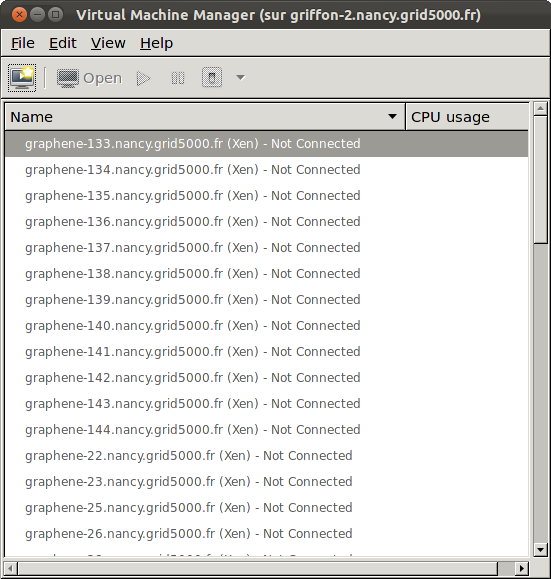
\includegraphics[width=300pt]{images/virt-ajout_noeuds.png}
\end{center}
Un simple clic sur un noeud établit la connexion puisque les mêmes clefs ssh ont étées copiées partout et le fichier \emph{known\_hosts} a également été répliqué pour éviter de confirmer l'ajout d'un hôte inconnue (opération qui devait se faire en ligne de commande car non gérée par virt).
\\
On est ensuite en mesure de créer une machine sur n'importe quel noeud, la procédure étant la même que pour une installation locale, nous n'allons pas la détailler à nouveau.

\subsection{Migration de machines}
Une fonctionnalité intéressate d'un gestionnaire de machines virtuelles est la migration des systèmes invités vers un autre hôte pour prévoir des opérations de maintenance, remplacement,...\\
Encore une fois virt-manger possède un outil graphique afin d'assister cette étape. Pour commencer, en effectuant un click droit sur une machine virtuelle on obitent un menu contextuel que nous allons détaillé au fur et à mesure.
\begin{center}
  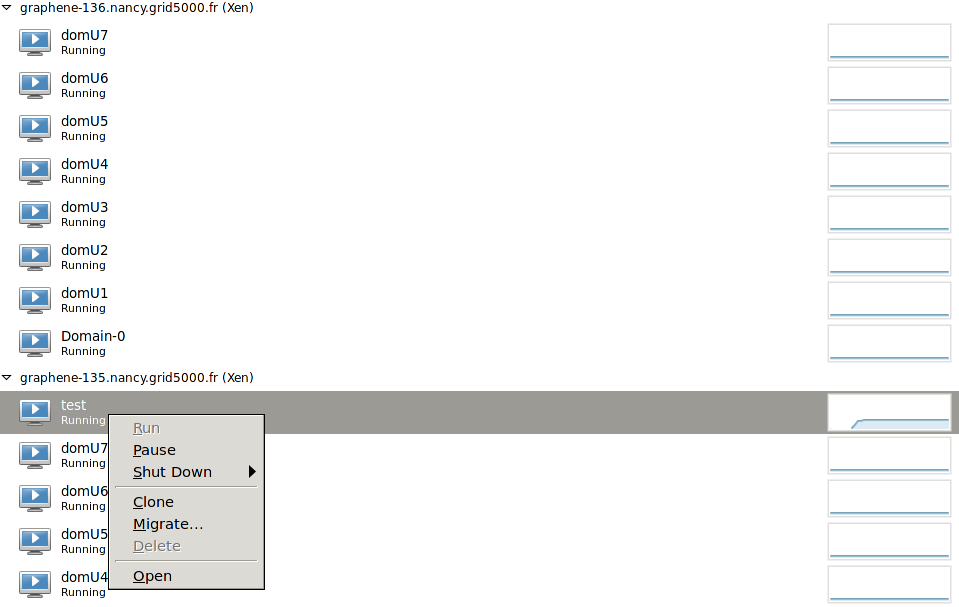
\includegraphics[width=350pt]{images/virt-menu-context.png}
\end{center}
En sélectionnant l'option \emph{Migrate} l'assistant demande alors sur quel autre noeud (préalamblement ajouté à virt) nous souhaitons transférer la machine virtuelle. L'opération peut prendre plusieures minutes en fonctions des capacités des machines et du réseau.
\begin{center}
  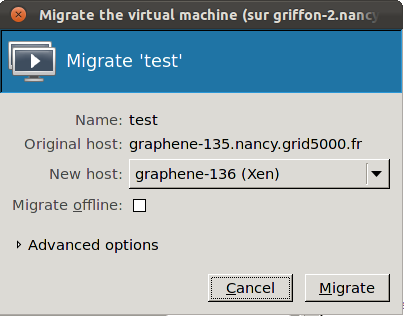
\includegraphics[width=250pt]{images/migration1.png}
\end{center}
\begin{center}
  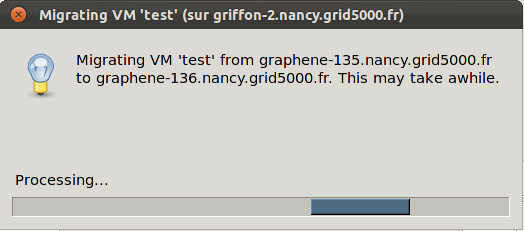
\includegraphics[width=250pt]{images/migration.png}
\end{center}

\appendix
\chapter{Sources}
\begin{description}
\item[www.grid5000.fr : ]le wiki disponible sur le site internet de grid5000 fut principale source de renseignements pour le démarrage du projet.
\item[www.loria.fr/\sim lnussbau/ : ]nous avons pu y consulter des anciens projets sur Grid5000 ce qui nous a permis d'avoir un premier aperçu de ses possibilités.

\end{description}

\chapter{Glossaire}
\begin{description}
\item[]
\item[]
\end{description}

\chapter{Scripts}
\section{réservation}
\lstset{language=ruby}
\begin{lstlisting}
puts "-----------------------------------------"
puts "Souhaitez vous reserver des noeuds?(y/n)"
loop do
  test = gets.chomp
  if test.eql?("n")
    puts "#####################"
    puts "#sortie du programme#"
    puts "#####################"
    break;
  end
  if test.eql?("y")
    #Reservation de machines                                                 
    puts "---------Script de reservation-----------"
    puts "Choisir un nombre de noeud:"
    noeuds = gets.chomp.to_i
    puts "Choisir un temps de reservation(HH:MM:SS):"
    temps = gets
    puts "\nVous avez reserve #{noeuds} noeuds 
	  pour une duree de #{temps}"
    puts "-----------------------------------------"
    exec "oarsub -I -t deploy -n'virtu' -l 
	  slash_22=1+nodes=#{noeuds},walltime=#{temps}"
    break;
  end
end
\end{lstlisting}

\newpage
\section{déploiment}
\begin{lstlisting}
#Deployer une image cree
puts "Voulez vous deployer une image?(y/n)"
loop do
  test = gets.chomp
  if test.eql?("n")
    puts "#####################"
    puts "#sortie du programme#"
    puts "#####################"
    break;
  end
  if test.eql?("y")
    #choix de l'image                                                                                                                 
    puts "-----------------------------------------------"
    puts "image disponibles:"
    puts `ls /home/\$USER/image | grep .env`
    puts "-----------------------------------------------"
    puts "Choix de la distibution(tout saisir):"
    debian = gets.chomp
    puts "-----------------------------------------------"
    exec"kadeploy3 -f \$OAR_FILE_NODES -a #{debian} -k 
	\$HOME/.ssh/id_rsa.pub"
    break;
  end
end
#Deploiment de l environement sur les noeuds reserves                          
puts "Voulez vous deployer un environement?(y/n)"
loop do
  test = gets.chomp
  if test.eql?("n")
    puts "#####################"
    puts "#sortie du programme#"
    puts "#####################"
    break;
  end
  if test.eql?("y")                                                            
    #choix de la version a deployer                                            
    puts "-----------------------------------------------"
    puts "distributions disponibles:"
    puts `kaenv3 -l | cut -d - -f1 | uniq | tail -n +3`
    puts "-----------------------------------------------"
    puts "Choix de la distibution:"
    debian = gets.chomp
    puts "-----------------------------------------------"
    puts "version de la distribution:"
    puts `kaenv3 -l | grep #{debian}| cut -d ' ' -f1`
    debian = debian+"-x64-"
    puts "-----------------------------------------------"
    puts "Choix de la version de la distribution a deployee 
	  (sans #{debian}):"
    version = gets.chomp
    version = debian+version
    puts version
    exec"kadeploy3 -e #{version} -f \$OAR_FILE_NODES -k 
	\$HOME/.ssh/id_rsa.pub"
    break;
  end
end
\end{lstlisting}

\section{configuration de base}
\lstset{
language=bash,
morekeywords{taktuk}
}
\begin{lstlisting}
########################################################
#------------------Configuration minimale--------------#
#______________________________________________________#

#recuperation des noeuds reserves
cat \$OAR_FILE_NODES | uniq  > \$HOME/script_base/list_nodes
list_nodes="\$HOME/script_base/list_nodes"

echo "-----------------------------------"
echo "Liste des machines reservee:"
cat \$list_nodes
echo "-----------------------------------"
echo "Copie des clees SSH vers toutes les machines."
for node in \$(cat \$list_nodes)
do
	scp \$HOME/.ssh/id_rsa* root@\$node:~/.ssh/
done
echo "-----------------------------------"

#mise a jour des noyaux
taktuk -l root -f \$list_nodes broadcast exec [ apt-get update ]
taktuk -l root -f \$list_nodes broadcast exec [ apt-get dist-upgrade 
      -q -y --force-yes ]
#changement des mdp root
taktuk -l root -f \$list_nodes broadcast exec [ 'echo -e 
      pttvirtu\npttvirtu" | passwd root' ]
\end{lstlisting}

\newpage
\section{Listing d'unne installation de Ganetti}
\begin{lstlisting}
#!/bin/bash
#passage en wheezy
rm /etc/apt/sources.list
echo "## wheezy security" > /etc/apt/sources.list
echo "deb http://security.debian.org/ wheezy/updates main contrib non-free" >> /etc/apt/sources.list
echo "deb-src http://security.debian.org/ wheezy/updates main contrib non-free" >> /etc/apt/sources.list
echo " " >> /etc/apt/sources.list
echo "#wheezy" >> /etc/apt/sources.list
echo "deb http://ftp.fr.debian.org/debian/ wheezy main contrib non-free" >> /etc/apt/sources.list
echo "deb-src http://ftp.fr.debian.org/debian/ wheezy main contrib non-free" >> /etc/apt/sources.list
#Installation de ganeti 
apt-get update
apt-get dist-upgrade -y --force-yes
apt-get install -y --force-yes ganeti2 ganeti-htools ganeti-instance-debootstrap
echo "Ajout du node dans /etc/hosts"
hostname=`cat /etc/hostname`
#recuperation des variables
#ip du node
ifconfig eth0 > troll
ipnode=`head -2 troll | tail -1 | cut -d':' -f2 | cut -d' ' -f1`
echo \$ipnode \$hostname >> /etc/hosts
#ip du broadcast
ipbroadcast=`head -2 troll | tail -1 | cut -d'B' -f2 | cut -d':' -f2 | cut -d' ' -f1`
#ip du masque de sous reseau
ipmask=`head -2 troll | tail -1 | cut -d'M' -f2 | cut -d':' -f2 | cut -d' ' -f1`
#ip du reseau
ipnetwork=`head -1 ipnetwork`
#ip de la passerelle
ipgateway=`head -1 ipgateway`
#ajout de cluster1 dans dans /etc/hosts
echo "ajout de cluster1 dans /etc/hosts"
ipcluster=`cat ipcluster`
echo \$ipcluster "cluster1" >> /etc/hosts
#Dans /boot/ creer des liens symboliques :
ln -s /boot/vmlinuz-2.6.32-5-xen-amd64 /boot/vmlinuz-2.6.xenU
ln -s /boot/initrd.img-2.6.32-5-xen-amd64 /boot/initrd.img-2.6.xenU
#Pour le moment changera surement.
echo "creation du LVM"
umount /dev/sda5
pvcreate /dev/sda5
vgcreate xenvg /dev/sda5
#Creation du bridge xen-br0
echo " " >> /etc/network/interfaces
echo "auto xen-br0"  >> /etc/network/interfaces
echo "iface xen-br0 inet static" >> /etc/network/interfaces 
echo "address" \$ipnode >> /etc/network/interfaces
echo "netmask " \$ipmask >> /etc/network/interfaces
echo "network" \$ipnetwork >> /etc/network/interfaces
echo "gateway"  \$ipgateway >> /etc/network/interfaces
echo "broadcast" \$ipbroadcast>> /etc/network/interfaces
echo "bridge_ports eth0" >> /etc/network/interfaces
echo "bridge_stp off" >> /etc/network/interfaces
echo "bridge_fd 0" >> /etc/network/interfaces
#Suppression des ligne de eth0
sed -i '9d' /etc/network/interfaces
sed -i '9d' /etc/network/interfaces
#supression des fichier temporaires
rm troll ipcluster  ipgateway  ipnetwork
#initialisation du cluster
gnt-cluster init --no-drbd-storage cluster1
#ajouter le node 
gnt-node add \$hostname
#et verifier
gnt-node list
\end{lstlisting}


\newpage
\subsection{Scripts pour le déploiement de virt-manager}
\lstinputlisting[language=bash]{scripts/virt-manager/config_base.sh}
\lstinputlisting[language=bash]{scripts/virt-manager/virt-install.sh}
\lstinputlisting[language=bash]{scripts/virt-manager/ajout_noeuds.sh}

\end{document}
